\documentclass[10pt,letterpaper]{article}
\pdfminorversion=7
\usepackage[margin=0.82in]{geometry}
\usepackage[T1]{fontenc}
\usepackage{lmodern}
\usepackage{array}
\usepackage{booktabs}
\usepackage{graphicx}
\usepackage{xcolor}
\setlength{\parindent}{0pt}
\setlength{\parskip}{6pt}
\begin{document}
\begin{center}
{\Large\bfseries Frob C5 direct-trace successor replay}\\[3pt]
{\small 25 October 2026 \quad $\vert$ \quad Exact frozen cells $q=11,13,19$}
\end{center}

\noindent\colorbox{green!12}{\parbox{\dimexpr\linewidth-2\fboxsep\relax}{\textbf{Mathematical result.} Direct repeated $q$-th powering of each quotient-basis element gives a five-term trace matrix $T$ equal to $h(M)$ in all three cells, with $h(X)=1+X+X^2+X^3+X^4$. Each $T$ has rank one and nullity four.}}

\section*{Two calculation paths}

The direct path uses polynomial convolution, monic long division modulo each frozen degree-five modulus, and repeated $q$-th powering. It constructs $T$ before reading or multiplying a Frobenius matrix. The second path evaluates $h$ on $M$ from the earlier source-bound matrix replay. The checker verifies SHA-256 hashes of that replay and each native output, then compares all 25 entries per cell.

\begin{center}
\small
\begin{tabular}{@{}lclcc@{}}
\toprule
Frozen cell & $q$ & Nonzero row of direct $T$ & Rank/nullity & $T=h(M)$ \\
\midrule
SPLIT & 11 & $[5,9,4,3,5]$ & $1/4$ & yes \\
NOLATTICE & 13 & $[5,5,12,8,1]$ & $1/4$ & yes \\
EQDEG & 19 & $[5,16,9,11,5]$ & $1/4$ & yes \\
\bottomrule
\end{tabular}
\end{center}

The remaining four rows are zero in every cell, so this direct trace lands in the base-field line. Its nullity equals the dimension recorded in the native C5 output.

\section*{Checks that can fail}

Changing the zero-based $(1,1)$ entry of the $q=13$ matrix from $2$ to $3$ makes $T\ne h(M_{\mathrm{mutant}})$. An injected bad native-output hash is rejected before arithmetic. The unmodified checker passes under ordinary Python and \texttt{python3 -O}; validation does not depend on disabled \texttt{assert} statements.

\section*{Historical boundary}

The original Sage output records a modulus and C5 flags, but does not serialize $M$. The prior replay reconstructs $M$ from the archived modulus. This successor calculation closes the direct-trace comparison for the pinned mathematical parameters, while the original subprocess's loaded driver and imports remain unauthenticated. The frozen historical C5 verdict remains \textbf{unestablished}. C8, the full success gate and all performance claims are outside this replay. No canonical performance graph value changes.

\vfill
\noindent\footnotesize Evidence: \texttt{recheck\_direct\_trace.py}, \texttt{replay.json}, and the repository's source-bound matrix replay. The full limitations and exact hashes are in \texttt{REPORT.md}.

\newpage
\section*{Evidence boundary diagram}

\begin{center}
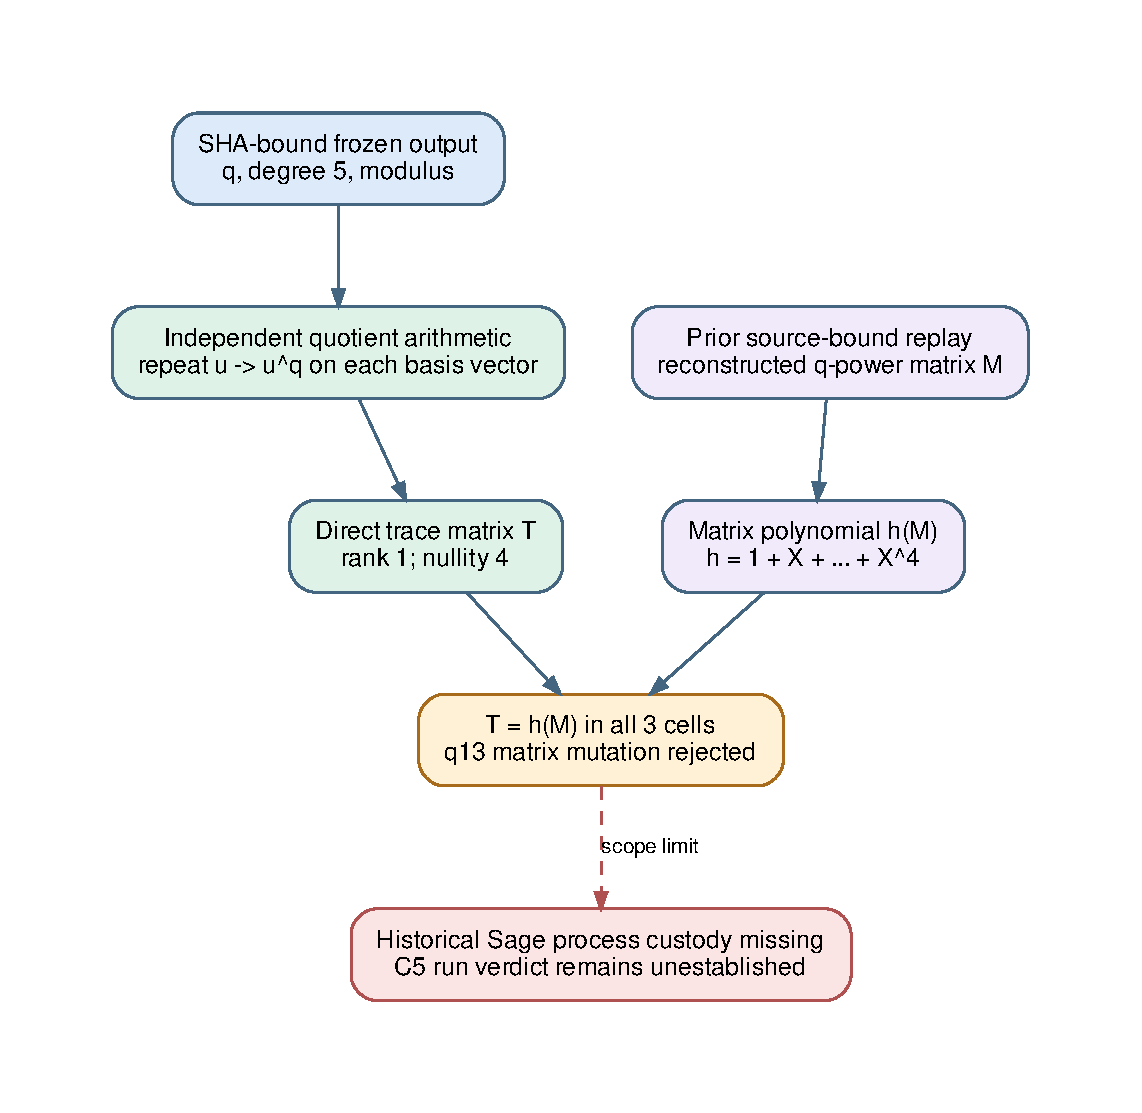
\includegraphics[width=0.89\linewidth,height=0.72\textheight,keepaspectratio]{trace-boundary-portrait.pdf}
\end{center}

The green path computes the direct trace without using a matrix. The purple path evaluates the matrix polynomial on the earlier source-bound replay's reconstructed $M$. Their equality is checked in the three frozen parameter cells, and the q13 matrix mutation fails. The dashed red boundary means this replacement mathematical replay cannot identify the code loaded by the original Sage subprocess.
\end{document}
